%Chapter describing the model
\chapter{The Model: Evolution of Mimicry}
\label{chapter:model}

\begin{quote}
\textsl{``Modeling, it should be clear is an art form. It depends on the experience and taste of the modeler. In this it is much like cartooning. The modeler (cartoonist) must decide which features to make salient (exaggerate), and which features to eliminate (avoid), in order to answer the questions (make the political point)" - John H. Holland \cite{holland1996}.}
\end{quote}

\section{Introduction}
%Entire section until past work needs to be revised when the model has been fully described.
The objective of this thesis is to design an agent based artificial life model for simulating the natural process of the evolution of mimicry.

There are mainly two species of agents. These agents have properties and behavior similar to the \textbf{model}, the \textbf{mimic} and the \textbf{predator} in the evolution of mimicry. We represent evolution of pattern for the model and the mimic with the help of Cellular Automata(CA). Cellular Automata can be easily represented by simple rules, which can be expressed as a binary string. The predator will be equipped with a Hopfield network, to be able to have pattern recognition capability. The process of evolution will of course be running at the genetic level. 

The choice of Hopfield Network memory for a predator can be considered appropriate as the number of patterns which can be recognized by this network is inversely proportional to the accuracy of recall. As more patterns are memorized, Hopfiled network tends to make more errors. This behavior will be appropriate for the simulation of Mullerian mimicry. Mullerian mimicry happens because of limited memory of the predators. Because of this limited memory, multiple inedible butterflies seems to converge to a single ring.

The environment is designed as three dimensional, while the space will be of toroidal nature. This idea has been taken from the \textsl{Laws and Life} project by Peter Grogono \cite{grogono2003}.

\section{Past Work}
Various models of mimicry has been simulated and explored. The model by Turner \cite{turner1996} and the mathematical model of Huheey \cite{huheey1988} tend to focus on the selective pressure on prey brought about by the particular learning abilities of the predator, and employ simple Monte Carlo or mathematical approaches.

Sherratt \cite{sherratt2002} provides an innovative perspective on the evolution of warning signals by considering co-evolving predator and prey populations. The model's predators are deterministic, in that they have a fixed behavioral strategy over their lifetime, and cannot learn from experience. For both cryptic and conspicuous prey, each predator has fixed policy of either attacking or avoiding.

The latest work on modeling evolution of warning signals and mimicry with individual based simulation is done by Frank and Noble. Their initial work \cite{franks2002} seems of focus on putting some conditions of mimetic evolution in an individual based model with multiple species preyed upon by a single abstract predator, where the appearance of each prey species can evolve but their palatability is fixed.

On 2003 \cite{franks2003} another model for the origin of mimicry ring has been proposed by Frank and Noble. Accordingly theory suggests that all Mullerian mimics in an ecosystem should converge into one large ring, while this convergence will be encouraged by presence of Batesian mimics. So an evolutionary simulation to observe the above mentioned phenomenon has been presented in this piece of work.

Frank and Noble continue to test the influence on mimicry ring evolution by Batesian mimics in their work on \cite{franks2004}. Usually mathematical models of mimicry has fixed prey coloration and appearances, which enables a comparison of predation rates to demonstrate the level of protection a mimic might be afforded. In this model prey colorations are free to evolve. This phenomenon is used to examine the effect of Batesian mimicry on Mullerian mimics and mimicry rings. 

\subsection{Models by Frank and Noble}
\label{subsec:models-by-frank-and-noble}
%Explain more about the first model by Frank and Noble
The \textbf{first} model by Frank and Noble \cite{franks2002} is where \textsl{``multiple species are preyed upon by a single abstract predator; the appearance of each prey species can evolve but their palatability is fixed"}. Each individual had a single gene: a value representing their external appearance or phenotype. The phenotypes are constrained to a ring of values from 1-20 (where 20 and 1 are neighbors). The distance of one phenotype from another represents their levels of similarity. 

A single abstract predator was modeled with a simple reinforcement learning system. The predator's experience of each phenotype was represented by a score, which would be maintained by probability to consume the next prey species depending on similarity or difference in phenotype. 

The existence of mimetic effect were measured with the initial and final distances between prey species' phenotypes. Three experiments were noted. Firstly, with one palatable and one unpalatable species. For this Batesian mimicry was evolved. For the second experiment, with two unpalatable species, Mullerian mimicry was evolved if the two prey species have some initial resemblance. Experiment 3 was carried out with two unpalatable and one palatable species, where the phenotype of the palatable species moved towards that of one of the unpalatable species, which is in other words Batesian Mimicry.

The \textbf{second} model by Frank and Noble \cite{franks2003} is based on two working hypothesis:

\begin{enumerate}
	\item \textsl{All of the Mullerian mimics in a given ecosystem should eventually converge into one large ring in order to gain maximum protection.}
	\item \textsl{If the Mullerian mimics do not converge into one large ring, then the presence of Batesian mimics could entice them to do so, by influencing the rings to converge.}
\end{enumerate}

Although there are many mathematical and stochastic models of mimicry in the biological literature, this model gives attention to the evolution of mimicry ring phenomenon from an artificial life perspective.

%\subsubsection{Model Description}
\paragraph{Prey}
Similar to the first model this also contains a population of prey species each having an appearance and palatability level. Different species of prey were each assigned a fixed palatability level on a scale between zero and one (least to most palatable), where 0.5 is neutrally palatable. Palatable species have values greater than 0.5, and unpalatable species have values lower than 0.5. Each prey species has used two genes with values compositely representing their external appearance or phenotype. Both of these genes were constrained to values from 1 - 200. The Euclidean distance of one phenotype from another represented their level of similarity.

\paragraph{Predator}
Similar to Turner's stochastic model \cite{turner_et_al1984},  predators were modeled with a Monte Carlo reinforcement learning system. The predator's experience of each phenotype was represented by an attack probability, which was initialized to ambivalence at 0.5. After eating prey of a particular phenotype, the predator would make a post-attack update of the relevant probability according to the palatability of the prey consumed. The predator would use its experience of different prey appearances to help it decide on whether or not to attack at the next opportunity.

In contrary to the stochastic model \cite{turner_et_al1984},  predators would generalize on the basis of experience. A set of probability formula was used to come up with the current probability to consume a prey species based on its palatability and the previous probability of consumption based on experience using generalization rate and the Euclidean distance between the experienced phenotype and the consumed prey phenotype. 

%Explain the results for the second model by Frank and Noble
\paragraph{Results}
According to the first experiment, which started with 20 unpalatable prey species, hypothesis 1 of a single large mimicry ring was not established. There was existence of multiple mimicry rings of very different frequency (population). Second experiment was carried out with some palatable species along with the unpalatable ones which was able to reach conditions of Batesian mimicry also with less mimicry rings, where hypothesis 2 borne out. It can be observed that,

\begin{quote}
\textsl{``The presence of Batesian mimics would provide positive selection pressure on mutants and would, therefore, increase the probability that they would evolve an initial resemblance to another unpalatable species. Also, Batesian pressure on mimicry rings has the potential to push one ring into the range of another, helping to bridge a large phenotypic difference between them." \cite{franks2003}}
\end{quote}

\section{FormAL Framework}
The \textsl{``FormAL framework"} is a collection of ideas and concepts taken from Peter Grogono's FormAL(Formal Artificial Life) project \cite{grogono2003} and are used to build a framework for modeling the evolution of mimicry. The primary goal of the FormAL project was ``\textit{To study the emergence of complexity}". While the principal behind it was ``\textit{not to include a variable in an agent unless the variable is genetically controlled (or, at least, genetically influenced)}". We will see that this principal was not completely established in simulating mimicry as it was not possible to come up with a genetic representation of Hopfield Network which was used as a pattern recognizer for the predator species. 

\subsection{Agents}
In FormAL, an \textbf{Agent} is a simulated organism. It is designed simply, but with the following qualities:

\begin{itemize}
	\item It has behaviors to be able to reproduce itself using genetic information.
	\item Capable of modifying the structure of genome between generations.
	\item Able to interact with other agents.
	\item And also to survive and reproduce in a challenging environment.
\end{itemize}

\subsection{Spatial representation of the environment}
The framework consists of a three dimensional visual environment where agents of the individual based simulation gets complete freedom of movement defined from their genetic representation. 

\paragraph{Space}
The space of the environment is a three-dimensional lattice of discrete points. The coordinate of each point in space is of the form \((x,y,z) \in \Sigma^3\), where \(\Sigma\) be the set \(\{0, 1, ..., S-1\}\). \(S\) is a universal constant being a small positive integer, which in this simulation has been kept at 20 (the value of the \(World Size\) parameter in table \ref{tab:environment-control-parameters}). 

\paragraph{Time}
Time, being an integer \( (t \geq 0) \), advances in discrete steps in the simulation, where at each step the agents update themselves. 

\paragraph{Cell}
The entire three dimensional toroidal environment is divided in multiple cells. A cell is a three dimensional cubical section of the hyperspace. Accordingly in table \ref{tab:environment-control-parameters} \(ISize\) is the parameter that controls the number of cells in the environment. The size of a cell is evaluated from the entire world size. And the total number of cell is calculated as \(ISize^3 = 216\).

\begin{table}[H]
\centering
\begin{tabular}{| p{2.2cm} | >{\centering} p{3cm} | p{7.5cm} |}
	\hline
		\textbf{Parameter} & \textbf{Value} & \textbf{Description} \\ \hline
		ISize & 6 & Number of cell in single dimension of the 3-D toroidal cube\\ \hline
		World Size & 20 & Size of a single dimension of the 3-D toroidal cube\\ \hline
		Cell Size & \( World Size / ISize \) & Size of each cell\\ \hline
		Total Number of Cells & \( ISize^3  = 216\) & Total number of cells in the environment\\ 
	\hline
\end{tabular}
\caption{Parameters to control the environment.}
\label{tab:environment-control-parameters}
\end{table}

\begin{table}[H]
\centering
\begin{tabular}{cc}
		\multicolumn{2}{c}{ 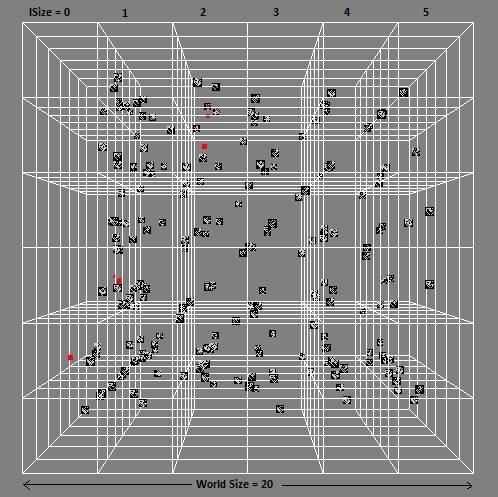
\includegraphics[scale=0.60]{images/cells-front} } \\
		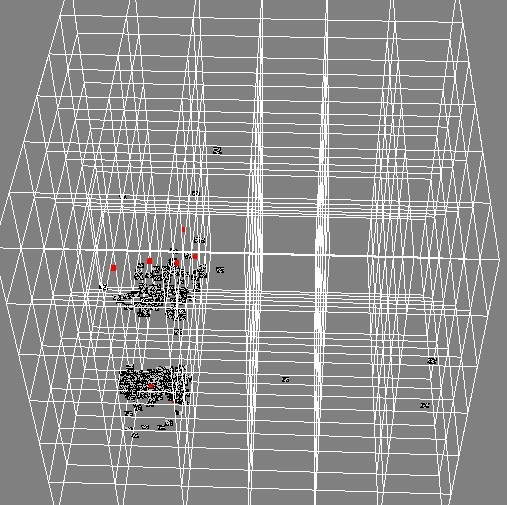
\includegraphics[scale=0.50]{images/cells-top} & 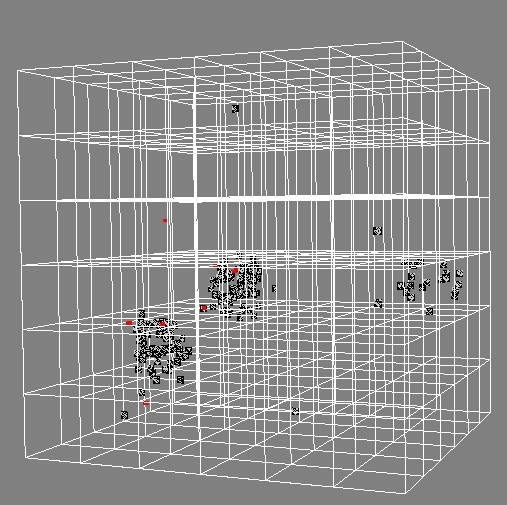
\includegraphics[scale=0.50]{images/cells-side} \\
\end{tabular}
\caption[Three dimensional representation of the environment]{Three dimensional representation of the environment divided in cells. Presence of different species of agents inside.}
\label{tab:3-d-environment-images}
\end{table}

\subsection{Mobility}
An agents position is calculated once during each step of update in time. The agents \(position\), \(force\), \(acceleration\) and \(velocity\) are all vector components. The \(force\) component is calculated from agent's mobility gene. And it is used to compute agent's \(acceleration\). If the \(force\) and \(velocity\) are both zero, then the agent has no effect in motion. Otherwise, Newton's law is used to obtain the \(acceleration\), which is integrated to obtain the new \(velocity\) and new \(position\).

\begin{algorithm}
	\caption{Algorithm for updating movement of the Agents}
	\label{algo:algorithm-movement-agents}
	\begin{algorithmic}
		\FOR{each step in time}
			\STATE $accelaration \gets ForceFactor * force - Friction * velocity$
			\STATE $velocity \gets DT*accelaration$ \COMMENT{DT is considered as Differential Time Set}
			\STATE $deltaPos \gets DT*velocity$
			\STATE $position \gets position + deltaPos$
		\ENDFOR
	\end{algorithmic}
\end{algorithm}

\begin{table}[H]
\centering
\begin{tabular}{| p{2.2cm} | >{\centering} p{1.3cm} | p{9cm} |}
	\hline
		\textbf{Parameter} & \textbf{Value} & \textbf{Description} \\ \hline
		Force Factor & 40 & A unit vector is multiplied by this amount before being added to the force vector.\\ \hline
		Differential Time Step (DT) & 0.01 & The time step used for first-order integration of the motion equations.\\ \hline
		Friction & 5 & The friction constant used for motion calculations.\\ \hline
		Work Factor & 1 & \( Work done = WF * force * distance \), where \(WF\) is this constant.\\
	\hline
\end{tabular}
\caption{Parameters to control mobility of agents.}
\label{tab:mobility-control-parameters}
\end{table}

Algorithm \ref{algo:algorithm-movement-agents} explains the calculation of mobility of each agent at each time step of the simulation, while table \ref{tab:mobility-control-parameters} contains the values of the parameters used to apply to this algorithm.

\section{The Prey: Mimics and Models}

\subsection{Pattern representation by Cellular Automata}
Only the significant characteristics which are required for a successful model of mimicry is implemented. As for this simulation we are considering heliconius butterfly, the representation of their wing pattern is with the help of cellular automata. So basically every prey organism will contain a genetic representation of cellular automata with which the predator will identify the prey and store its level of palatability in memory.

%More content needs to be added for cellular automata.
\subsubsection{Cellular Automata}

Cellular automata are computer generated patterns applying very simple rules. First invented by Jon von Neuman and later extended by Stephen Wolfram, this field of study has created a lot of enthusiasm in the evolution of complexity with blocks of simplicity, in this case rules. We choose cellular automata as it can be easily represented with the help of a binary genome and then evolutionary operations on the genomic representation, such as mutation and crossover can easily be applied.

\begin{figure}[H]
	\centering
	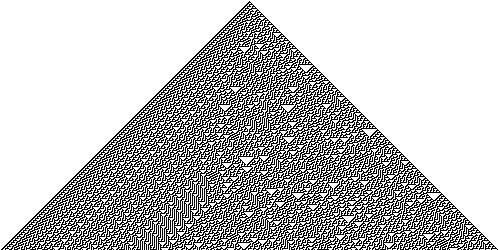
\includegraphics[scale=5]{images/CA_rule30s}
	\caption[Cellular Automata]{Cellular Automata Rule 30.
	Image source: \href{http://en.wikipedia.org/wiki/Cellular_automata}{Wikipedia}}
	\label{fig:cellular-automata-rule-30}
\end{figure}

\begin{table}[H]
	\centering
	\begin{tabular}{| l | c | c | c | c | c | c | c | c |}
	  \hline
	  Current Pattern & 111 & 110 & 101 & 100 & 011 & 010 & 001 & 000 \\ \hline
	  New state of center cell & 0 & 0 & 0 & 1 & 1 & 1 & 1 & 0 \\
	  \hline
	\end{tabular}
	\caption{Cellular Automata rule}
	\label{tab:cellular-automata-rule}
\end{table}

In generating the pattern of Figure \ref{fig:cellular-automata-rule-30}, the genetic representation would be the 'New state of center cell'. As Figure \ref{fig:cellular-automata-rule-30} is a rule 30 cellular automata, the eight bit binary representation of 30 would be the genetic representation for this pattern. Generation of automata pattern from this binary string can be considered analogous to the complex pathway between the genotype and the phenotype that exists in all living organism.

\subsection{Species diversity}
Franks and Noble have used different models to diversify species. In \cite{franks2002} they have used linear difference in number ``constrained to a 'ring' of values  from 1-20 (where 20 and 1 are neighbors)" to distinguish species diversity. Here the distance of one phenotype from another represents their level of similarity. 

To use CA as prey pattern, an agent's genome is constructed as an 8 bit binary value with a decimal range between 0 to 255. Each of this 256 values have a unique CA pattern associated with it. When storing this pattern in Hopfield memory we take a linear representation of this 2-D pattern, while to consider similarity between two pattern we evaluate the hamming distance between their linear representation. 

With CA based pattern representation, population of prey species with a specific CA pattern can be grouped as one single species. And by restricting inter species reproduction we can control the diversity of patterns. But there is mutation applied when similar species mate with each other, so new species do born out of generations of existing species. So that is why we have two separate mutation rate while reproducing prey species. One being the ``Pattern Mutation Rate" (default values are mentioned in table \ref{tab:prey-control-parameters}) with which we control mutation of the first 8 bits of the genome while the ``Genome Mutation Rate" is used to control mutation of rest of the 9 bit genome (table \ref{tab:prey-genome}). Similar efforts of multiple mutation rate at varying location has been used in developing ``Echo" as mentioned in section \ref{subsec:echo} \cite{hraber1997}.

\subsection{Genome}
The Genome of the prey species consists of 17 bits as presented in table \ref{tab:prey-genome}. The first eight bits is the rule, which is used to generate Cellular Automata pattern. The next two bits are used to represent palatability of the organism explained detail in section \ref{sec:genetic-palatability-representation}. The next six bits is the magnitude of the force with which mobility of the organism is calculated. The 17th bit is used to evaluate reproduction capability of the organism, depending on which the prey species is either capable or not capable to participate in reproduction.

\begin{table}[H]
\centering
\begin{tabular}{|c|c|c|c|}
	\hline
		\textbf{Pattern(8)} & \textbf{Palatability(2)} & \textbf{Mobility(6)} & \textbf{Reproduction(1)} \\ \hline
		10101101					 	& 							01		 		 & 			110001					&					1						 		 \\ \hline
\end{tabular}
\caption{Distribution and purpose of each gene of the 17 bit prey genome.}
\label{tab:prey-genome}
\end{table}

\subsection{Reflection of punctuated equilibrium}
\label{subsec:reflection-of-punctuated-equilibrium}
Punctuated equilibrium has been defined in section \ref{sec:evolutionary-dynamics-of-mimicry} as the evolutionary process that is more inclined to cladogenesis instead of gradualism. Also Turner \cite{turner1988} emphasizes on punctuated equilibrium to describe the evolution of mimicry instead of phyletic gradualism. The design of the model under discussion also follows Turner's explanation in terms of evolving mimicry. As it can be observed new CA patterns evolve from existing ones in prey population just by a single mutation in the pattern gene. Mimics do not follow a gradual process of evolution to look close to models but rather the change happens randomly through a single step mutation. The mutations that are favored, helps the mimics to survive while the unfavored ones fail to persist. It can be observed later in table \ref{tab:diff-in-pattern} how CA patterns of prey species can have vastly different configuration for a unit change in their representative gene. 

\subsection{Genetic representation of palatability}
\label{sec:genetic-palatability-representation}
The palatability of each prey species is fixed and has been represented with 2 bits of the genome giving it a range of 0 to 3 with four levels of palatability. The combinations are as follows:

\begin{table}[H]
	\centering
	\begin{tabular}{|c|c|}
		\hline
			\textbf{Gene (Index 8 to 9)} &	\textbf{Palatable} \\ \hline
			00									& True 			\\ \hline
			01									& True 			\\ \hline
			10									& False 		\\ \hline
			11									& False 		\\
		\hline
	\end{tabular}
	\caption{Genetic representation of palatability}
	\label{tab:genetic-representation-palatability}
\end{table}

This representation in table \ref{tab:genetic-representation-palatability} is unlike Frank and Noble \cite{franks2003} where palatability level has been used on a scale between zero and one (least to most palatable), where 0.5 is neutrally palatable. 

\subsection{Interaction between other Prey and Predators}
The prey have been defined to have many conglomerate behavior in the environment. Prey interaction with other prey species and with predators make the evolution of mimicry possible. Mobility of prey species and their reproduction capability are two important behaviors which result from interaction. 

\subsubsection{Mobility}
The mobility genes of the prey consist of 6 bits. These six bits are used to calculate the force with which each prey try to move towards any neighborhood cell. The algorithm sorts all neighboring cell descending to the number of prey species. Then it selects the cell which contains the highest number of prey with zero predator. If all the neighboring cells contain predators, then the algorithm sorts the neighboring cells descending on the number of predators and chooses the one which contains the least. Algorithm \ref{algo:algorithm-movement-prey} explains in detail.

\begin{algorithm}[H]
	\caption{Algorithm for updating position of the Prey species}
	\label{algo:algorithm-movement-prey}
	\begin{algorithmic}
		\FOR{each step in time}
			\STATE $forceMagnitude \gets convertToDecimal(genome[10-15])$
			\STATE Get list of neighborhood cells, sorted by population of prey species.
			\STATE From the sorted cell list choose the one with the least number of predators and most number of prey.
			\STATE Move towards the selected cell with $forceMagnitude$ unit of force.
		\ENDFOR
	\end{algorithmic}
\end{algorithm}

\subsubsection{Reproduction}
Every prey species starts reproducing when it reaches the \textsl{``Reproductive age limit"}. If it is capable of reproducing, which is decided based on its 17th bit gene, the prey will randomly select another prey species with similar pattern and palatability from the same cell and mate with it. Now the other prey also needs to be genetically capable of reproduction and needs to reach its age limit. A new genome is created from the existing genome of the two prey by applying single point crossover operation. Mutation is performed separately on the pattern gene and the rest of the genome, with two different rates to control them using the values in table \ref{tab:prey-control-parameters}. So there is two point mutation for the genome. 

\begin{algorithm}[H]
	\caption{Algorithm for reproduction of the Prey species}
	\label{algo:algorithm-reproduction-prey}
	\begin{algorithmic}
		\FOR{each step in time}
			\STATE $capableToReproduce \gets$ true or false depending on the 17th bit of the genome, and maturity on reproduction age.
			\IF {$capableToReproduce == true$ and $currentCellPopulation > 1$ } 
				\STATE $anotherPrey \gets$ Select random prey from same cell.
				\IF {$anotherPrey$ is alive and $capableToReproduce$ and of similar $pattern$ and $palatability$}
					\STATE Perform genetic cross over and mutation to create new genome.
					\STATE Create new prey with new genome, and release into environment.
					\STATE Record reproduction time for both prey.
				\ENDIF
			\ENDIF
		\ENDFOR
	\end{algorithmic}
\end{algorithm}

\begin{table}[H]
\centering
\begin{tabular}{| p{2.2cm} | >{\centering} p{1.5cm} | p{9cm} |}
	\hline
		\textbf{Parameter} & \textbf{Value} & \textbf{Description} \\ \hline
		Prey Size & 2 to 5 & Size of the prey species in the 3D FormAL  environment.\\ \hline
		Reproduction age limit & 100 & Minimum number of iterations or time steps a prey species need to be present in the simulation to get reproduction capability\\ \hline
		Reproduction interval & 1000 & Number of iterations a prey need to wait before reproducing again.\\ \hline
		Pattern Mutation Rate & 0.05 & Rate of Mutation of the pattern genome.\\ \hline
		Genome Mutation Rate & 0.5 & Rate of mutation of the rest of the genome excluding the pattern gene.\\ \hline
		Demise Age & 2000 & Age at which the prey species will be removed from the environment.\\
	\hline
\end{tabular}
\caption{Parameters to control prey population and visibility.}
\label{tab:prey-control-parameters}
\end{table}

\section{Predator}

Predators in the system are designed to provide selection pressure to \textit{models} and \textit{mimics} for the evolution of mimicry. Similar to prey species, they are agents in the FormAL environment capable of mobility and reproduction. In addition to it, these agents are equipped with Hopfield Network Memory to be able to learn and recognize patterns of the prey species. Their mobility and reproduction capability is controlled at the genetic level, while their memory is not genetically controlled, as it was not possible to come up with a genetic representation for Hopfield Network. So every new predator species gets to born with zero memory and with no inheritance from parents. A set of parameters are defined to control predators' population and learning ability in the environment. Details of these parameters are given in table \ref{tab:predator-control-parameters}.

\subsection{Learning}
The objective of a predator's interaction with prey is always to consume it. But based on the prey's pattern and palatability, the predator will either be able to consume it or throw it back to the environment. At this event the predator needs to learn the pattern with which the prey has been represented. The pattern represents palatability of the prey species, at least to the predator. To store this new pattern into memory, each predator is equipped with a Hopfield Network Memory. Every time a new interaction is made by the predator its memory is initialized with all the existing pattern that has already been encountered and the new one. The learning procedure used for this memory is Hebbian Learning. 

\subsubsection{Hebbian Learning}
\textit{Hebb's postulate of learning} is the oldest and most famous of all learning rules; it is named in honor of the neuropsychologist Donald Hebb(1949). Hebb's book \textit{The Organization of Behavior} \cite{hebb1949} states the following:

\begin{quote}
\textsl{``When an axon of cell A is near enough to excite a cell B and repeatedly or persistently takes part in firing it, some growth process or metabolic changes take place in one or both cells such that A's efficiency as one of the cells firing B is increased."}
\end{quote}

The following \textit{general learning rule} is adopted in neural network studies: \textit{The weight vector} \( \textbf{w}_i = [w_{i1} \> w_{i2} \> ... \> w_{in}]^t \) \textit{increases in proportion to the product of input} \textbf{x} \textit{and learning signal r}. The learning signal r is in general a function of \(\textbf{w}_i,\textbf{x}\), and sometimes of the teacher's signal \(d_i\). Thus we have, 
\begin{equation}
	r = r(\textbf{w}_i,\textbf{x},d_i)
%\label{eq:}
\end{equation}
The increment of the weight vector \(\textbf{w}_i\) produced by the learning step at time t according to the general learning rule is,
\begin{equation}
	\Delta\textbf{w}_i(t)=cr[\textbf{w}_i(t),\textbf{x}(t),d_i(t)]\textbf{x}(t)
%\label{eq:}
\end{equation}
when c is a positive number called the \textit{learning constant} that determines the rate of learning.

For Hebbian learning rule the learning signal is equal simply to the neuron's output. We have
\begin{equation}
	r \overset{\Delta}{=} f(\textbf{w}_i^t \textbf{x})
%\label{eq:}
\end{equation}
The increment \(\Delta\textbf{w}_i\) of the weight vector becomes
\begin{equation}
	\Delta\textbf{w}_i = cf(\textbf{w}_i^t \textbf{x})\textbf{x}
%\label{eq:}
\end{equation}
The single weight \( w_{ij} \) is adapted using the following increment:
\begin{equation}
	\Delta\textit{w}_{ij} = cf(\textbf{w}_i^t \textbf{x})x_j
%\label{eq:}
\end{equation}
This can be written briefly as 
\begin{equation}
	\Delta\textit{w}_{ij} = c o_i x_j, \> \text{for} \> j = 1, 2, ..., n
%\label{eq:}
\end{equation}
The learning rule requires the weight initialization at small random values around \( \textbf{w}_i = \textbf{0}\) prior to learning. The Hebbian learning rule represents a purely feed-forward, unsupervised learning. The rule implements the interpretation of the classic \textit{Hebb's postulate of learning} stated above. 

The rule states that if the cross product of output and input, or correlation term \(o_ix_j\) is positive, this results in an increase of weight \(w_{ij}\); otherwise the weight decreases. It can be seen that the output is strengthened in turn for each input presented. Therefore, frequent input patterns will have most influence at the neuron's weight vector and will eventually produce the largest output.

Training for Hopfield Network used for predator's memory is done by Hebbian Learning. Initially the weights are all set to zero. Using Hebbian rule, the outer product of the input - output vector pairs are calculated for each pattern. As Hopfield is a feedback network, the output of the network is also the input. The outer vector matrix of all the patterns are summed to come up with the final weight matrix. Each component of the weight matrix \(\textbf{W} = \{w_{ij}\}\) is given by:
\begin{equation}
w_{ij} = \sum_{p=1}^{P} s_i(p) t_j(p), i \neq j
%\label{eq:}
\end{equation}
\[
w_{ij} = 0, i = j
\]
where P is the number of patterns. Vectors \textbf{S} and \textbf{T} are respectively, the input and the desired output of the network.

\subsection{Design of Memory with Hopfield Network}

\subsubsection{Hopfield Network}

Algorithm for the Hopfield model is described in the following:

\begin{enumerate}
	\item \textit{Learning.} Let \( \boldsymbol{\xi}_1, \boldsymbol{\xi}_2, ..., \boldsymbol{\xi}_{\mu} \) denote a known set of N-dimensional fundamental memories. Use the outer-product rule (i.e. Hebb's postulate of learning) to compute the synaptic weights of the network as 
	\begin{equation}
		w_{ji} =
			\begin{cases}
				\frac{1}{N} \sum_{\mu=1}^{M}\xi_{\mu,j}\xi_{\mu,i}	& j \neq i \\
				0																										& j = i 
			\end{cases}
	%\label{eq:}
	\end{equation}
	where \(w_{ji}\) is the synaptic weight from neuron \(i\) to neuron \(j\). The elements of the vector \( \boldsymbol{\xi}_\mu \) equal \(\pm 1\) (bipolar). Once they are computed, the synaptic weights are kept fixed.
	
	\item \textit{Initialization.} Let \( \boldsymbol{\xi}_{probe} \) denote an unknown N-dimensional input vector (probe) presented to the network. The algorithm is initialized by setting
	\begin{equation}
		x_j(0) = \xi_{j,probe}, \> j = 1,...,N
	%\label{eq:}
	\end{equation}
	where \( x_j(0) \) is the state of neuron \(j\) at time \(n = 0\) and \( \xi_{j,probe} \) is the \(j\)th element of the probe \( \boldsymbol{\xi}_{probe} \).
	
	\item \textit{Iterate Until Convergence.} Update the elements of state vector \( \boldsymbol{x}(n) \) asynchronously (i.e., randomly and once at a time) according to the rule
	\begin{equation}
		x_j(n+1)=sgn \Bigg(\sum_{i=1}^{N} w_{ji}x_i(n) \Bigg), \> j = 1,2, ..., N
	%\label{eq:}
	\end{equation}
	Repeat the iteration until the state vector \( \boldsymbol{x} \) remains unchanged.
	
	\item \textit{Outputting.} Let \( \boldsymbol{x}_{fixed} \) denote the fixed point (stable state) computed at the end of the step 3, The resulting output vector \( \boldsymbol{y} \) of the network is
	\begin{equation}
		\boldsymbol{y} = \boldsymbol{x}_{fixed}
	\label{eq:}
	\end{equation}
	Step 1 is the storage phase, and steps 2 through 4 constitute the retrieval phase.
\end{enumerate}

%This section needs to use similar variables as mentioned in the above section on Hopfield Network.
\subsubsection{Input to memory}
Each prey contains an evolving cellular automata which is represented by a binary gene. This two dimensional pattern is serialized to be available as a one dimensional binary array, which is taken as input for any predator organism trying to interact with the prey. This binary representation of the pattern gets converted to a bipolar representation. Each input pattern will consist of \(\textit{m} \times \textit{n} = \textit{mn}\) components, each component representing one pixel of the pattern (\textit{m} and \textit{n} representing each dimension). The \textit{m} by \textit{n} pattern configuration will be serialized by putting all row vectors in one single row sequentially.

\subsubsection{Predator attack algorithm}
As soon as a predator reaches its attack age it selects random prey species around its vicinity and starts attacking them. This attack process also involves recognition of prey pattern, which is at the heart of mimicry simulation for this research. Two parameters have been defined to limit predator memorization and recognition process as both of these processes are computationally expensive. The ``Hopfield Minimum Memory Size" (default value in table \ref{tab:predator-control-parameters}) is the number of memory a predator needs to store before making intelligent decisions about attacking a new prey species. After a predator is born, it start attacking prey without any caution. But after every attack the predator will store its pattern and palatability level inside its memory. As soon as it reaches the minimum memory size, it will start making intelligent decision about attacking the next species. It will try to recognize the pattern and if found palatable, prey will be consumed. Otherwise prey will be thrown back into the environment. If the pattern is not recognized predator will try to consume it and in the process will store its palatability and pattern into memory. 

In this way the predator memory is limited to \textsl{``Hopfield Maximum Memory Size"}. After reaching this memory predator will not store any more new pattern but will try to associate with the existing ones it has already stored. Algorithm \ref{algo:algorithm-attack-prey} and \ref{algo:algorithm-attemptToKill} explains the process in every detail.

\begin{algorithm}
	\caption{Algorithm for attacking Prey species}
	\label{algo:algorithm-attack-prey}
	\begin{algorithmic}
		\FOR{each step in time}
			\IF {Predator has reached Minimum attack age}
				\STATE $preyToAttack \gets$ select random prey species from the same cell.
				\IF {$currentMemorySize < MinimumMemorySize$}
					\STATE $attemptToKill(preyToAttack);$ \COMMENT {Function defined in Algorithm \ref{algo:algorithm-attemptToKill}}
				\ELSE
					\STATE recognize $preyToAttack$ pattern from memory.
					\IF {prey is not recognized or prey is palatable}
						\STATE $attemptToKill(preyToAttack)$
					\ELSE 
						\STATE Prey is recognized as unpalatable, so release it back into environment.
					\ENDIF
				\ENDIF
			\ENDIF
		\ENDFOR
	\end{algorithmic}
\end{algorithm}

\begin{algorithm}
	\caption{$attemptToKill(preyToAttack)$}
	\label{algo:algorithm-attemptToKill}
	\begin{algorithmic}
		\STATE Kill $preyToAttack$.
		\IF {Memory size $< MaxMemorySize$}
			\STATE Associate $preyToAttack$ pattern and palatability and store into memory.
			\STATE Recalculate Hopfield Memory Weights using Hebbian Learning outer product rule.
		\ENDIF
	\end{algorithmic}	
\end{algorithm}

\subsection{Genome}
Each predator has a 5 bit genome as explained in table \ref{tab:predator-genome}. The first 4 bits represent its mobility and magnitude of the force component with which it moves around the environment. The last bit controls reproduction capability of each species.

\begin{table}[H]
\centering
\begin{tabular}{|c|c|}
	\hline
		\textbf{Mobility(4)} & \textbf{Reproduction(1)} \\ \hline
				 1101					   &					1						 		\\ \hline
\end{tabular}
\caption{Distribution and purpose of each gene of the 5 bit predator genome.}
\label{tab:predator-genome}
\end{table}

\subsection{Mobility and reproduction capability}
Movement behavior of a predator is calculated from its genome. The first 4 bits of the genome are converted from binary to decimal to determine the magnitude of force at which it will move towards the maximum crowd of prey present within its neighborhood. So magnitude of movement of a predator varies within a range of 0-15 units. If no prey is present in the neighborhood then this force is active in trying to keep predators distributed all over the cells. A predator chooses the neighborhood cell which contains the least number of predators. When the neighborhood contains zero predators, it would select any one of them randomly and move towards that cell.

\begin{algorithm}[h]
	\caption{Algorithm for updating position of the Predator species}
	\label{algo:algorithm-movement-predator}
	\begin{algorithmic}
		\FOR{each step in time}
			\STATE $forceMagnitude \gets convertToDecimal(genome[0-3])$
			\STATE Get list of sorted neighborhood cells. Sorted by population of prey species.
			\STATE From the sorted cell list choose the one with the least number of predators and most number of prey.
			\STATE Move towards the selected cell with $forceMagnitude$ unit of force.
		\ENDFOR
	\end{algorithmic}
\end{algorithm}

\begin{figure}[H]
	\centering
	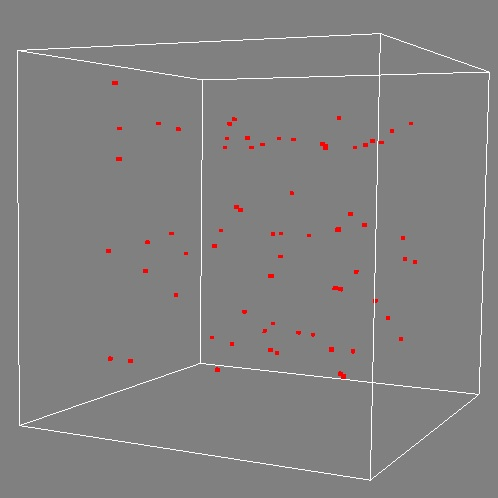
\includegraphics[scale=0.60]{images/predators-40}
	\caption[A population of predators]{A population of 40 predators distributed over the environment.}
	\label{fig:predators-40}
\end{figure}

The screen shot in Figure \ref{fig:predators-40} is from the simulation with only 40 predator species. It is presented to show the behavior of predator species in the simulation in absence of any prey species. As it can be observed the predators are distributed all over the cells with a constant mobile behavior to switch to another neighboring cell depending on which ever contains the least number of predator and also most number of prey species. This behavior of predator has been designed to enforce the predatory behavior of these agents and also to have increased predator prey interaction in the simulation in terms of one agent chasing the other for survival of species. 

\subsection{Reproduction process}
The  fifth gene of the predator is used to represent their capability of reproduction.  Depending on its binary value a predator in the simulation will or will not be able to reproduce. The reproduction process for predators is similar to prey species. As the learning capability of predators do not have any genetic representation, only the mobility behavior and reproduction capability takes effect in the reproductive process from one generation to another. 

There are two control parameters that effect the reproduction of predator species. The first is \textsl{``Reproduction Age Limit"}. This is the minimum age a predator has to reach before starting to involve itself for reproduction. This parameter has been set to 500 iterations during the result and analysis section of the thesis. The second parameter is \textsl{``Reproduction Interval"} which has been varied in the simulation from 1000 to 3000 iteration depending on the population of palatable prey species. This is a very important parameter for the simulation as it determines the overall predator population and its rate of increment. Depending on this value we can control the rate of predation on prey species, which on the other hand controls the rate of mimetic behavior of the overall prey population.

\begin{algorithm}[H]
	\caption{Algorithm for reproduction of the Predator species}
	\label{algo:algorithm-reproduction-predator}
	\begin{algorithmic}
		\FOR{each step in time}
			\STATE $capableToReproduce \gets$ true or false depending on the 5th bit of the genome, and maturity on reproduction age.
			\IF {$capableToReproduce == true$ and $currentCellPopulationOfPredators > 1$ } 
				\STATE $anotherPredator \gets$ Select random predator from same cell.
				\IF {$anotherPredator$ is alive and $capableToReproduce$ and also reached reproduction maturity age}
					\STATE Perform genetic cross over and mutation to create new genome.
					\STATE Create new predator with new genome and zero memory, and release into environment.
					\STATE Record reproduction time for both predators.
				\ENDIF
			\ENDIF
		\ENDFOR
	\end{algorithmic}
\end{algorithm}

When the above two conditions are met, meaning the predator reaches its age for reproduction and also crosses its age interval, it randomly select another predator residing in the same cell. If this random predator is capable to reproduce depending on its 5th gene, then with a random single point crossover and mutation a new predator species in born which also resides on the same cell and initializes with zero memory configuration. Similarly when the new born predator reaches its maturity of reproductive age and if it is capable of reproduction then the process iterates itself. 

\begin{table}[H]
\centering
\begin{tabular}{| p{2.2cm} | >{\centering} p{2.2cm} | p{8cm} |}
	\hline
		\textbf{Parameter} & \textbf{Value} & \textbf{Description} \\ \hline
		Minimum Memory Size & 2 to 6 & Minimum number of patterns stored in memory before predators start making intelligent decisions.\\ \hline
		Maximum Memory Size & 10 & Maximum number of patterns to be stored in memory. Limited to reduce processing time. \\ \hline 
		Hopfield Maximum Iterations & 20 & Maximum number of iterations for Hopfield Network to recognize a pattern. Usually the network reaches a steady state before that. But this restriction is to avoid infinite loop in case the network never reaches a steady state. \\ \hline
		Attack Age & 500 & minimum age a predator needs to reach to be able to attack prey species.  \\ \hline
		Attack Interval & 100 & Interval of time which needs to pass before a predators attacks its next prey. \\ \hline
		Genome Mutation rate & 0.3 & Mutation rate for the 5 bit genome of the predators representing their mobility and pattern recognition capability. \\ \hline
		Reproduction Age Limit & 500 & Minimum age a predator needs to reach before engaging in reproduction.\\ \hline
		Reproduction Interval & 1000 to 3000 & Interval of time a predator needs to pass between two reproduction process.\\ \hline
		Demise Age & 2000 to 7000 & Age at which a predator is considered as dead.\\
	\hline
\end{tabular}
\caption{Parameters to control predator population and pattern recognition capability.}
\label{tab:predator-control-parameters}
\end{table}

\section{Conclusion}
This model has been designed from a practical point of view; to come up with efficient results and achieve the main objective, \textit{evolution of mimicry}. Creation and transformation of different mimicry ring and also the dynamics of it has been integrated to achieve interesting results. This model can also be considered as a complex adaptive system similar to Hollands work on ``Echo" \cite{holland1996}. The seven basics of a complex adaptive system which are: Aggregation, Tagging, Nonlinearity, Flow, Diversity, Internal Models and Building blocks are present in this model.